\documentclass[12pt, openany]{book}
\usepackage{graphicx} % Required for inserting images
\setlength\parindent{0pt} % Remove default indentation
\setcounter{tocdepth}{2} % Remove subsubsections and below from contents

\usepackage{url}
\usepackage{listings}
\usepackage{color}
\usepackage{subcaption} % for subfigures

\usepackage{blindtext}
\usepackage{geometry}
 \geometry{
 a4paper,
 total={170mm,257mm},
 left=25mm,
 right=25mm,
 top=25mm,
 }
 
\usepackage{fancyhdr}
\pagestyle{fancy}
\lhead{%
    Computational Efficiency of PINN-based Approximations of Oscillating Systems
    }
\rhead{J.D.}
\renewcommand{\headrulewidth}{0.4pt}
 
\definecolor{dkgreen}{rgb}{0,0.6,0}
\definecolor{gray}{rgb}{0.5,0.5,0.5}
\definecolor{mauve}{rgb}{0.58,0,0.82}

\lstset{frame=tb,
  language=Python,
  aboveskip=3mm,
  belowskip=3mm,
  showstringspaces=false,
  columns=flexible,
  basicstyle={\small\ttfamily},
  numbers=none,
  numberstyle=\tiny\color{gray},
  keywordstyle=\color{blue},
  commentstyle=\color{dkgreen},
  stringstyle=\color{mauve},
  breaklines=true,
  breakatwhitespace=true,
  tabsize=3
}

\title{\LARGE %
        Computational Efficiency of PINN-based Approximations of Oscillating Systems \\
        \Large
        \vspace{15pt}
        School of Electronic Engineering and Computer Science \\
        \vspace{15pt}
        Final Report
        \vspace{30pt}
        \vfill
        }

% https://www.london.ac.uk/media/11184

\author{%
        \Large
        
\includegraphics[width=10cm]{Queen-Mary-logo.jpg} \\
        \vspace{15pt} \\
        Programme of Study: BSc Computer Science \\
        Supervisor: Dr Johan Pauwels \\
        Student: James Davies \\
        }
\date{Submitted: 29th April 2024}

\begin{document}

\maketitle

% ------------------------------------------------------- %

\thispagestyle{empty}
\chapter*{Abstract}

Approximating solutions to the complex mathematical equations that underpin our physical systems is an incredibly energy-intensive process. Finding solutions to these equations becomes increasingly difficult as dimensionality increases and data becomes more sparse, with the scientific community turning to machine learning (ML) methods to try and alleviate these issues. Approximations of Ordinary Differential Equations (ODEs) and Partial Differential Equations (PDEs) via traditional methods are both faster and more accurate, but computationally expensive. ML-based methods have the potential to offer efficient, scalable and real-time approximations to these equations, with the environmental cost of simulations/training models under scrutiny as the impact of high-performance computing on the environment is evaluated. From a climate perspective, improving computational efficiency in regard to resource utilisation also becomes important for increasing the accuracy of modelling complex and nonlinear physical systems; allowing researchers to develop more powerful physics-based models for ocean surface or climate modelling. \vspace{13pt}

This report focuses on one proposed solution for a generalised solution for solving ODEs and PDEs, named physics-informed neural networks (PINNs). This extension of artificial neural networks (ANNs), whilst benefiting from real-time approximations, is simple in its implementation, easy to parallelise using ML-libraries and can be run directly on graphics processing units (GPUs). Their implementation involves an extension of a fully-connected neural network (FCNN), via an added term of the loss function. PINNs utilise the prior knowledge of physical systems by calculating the PDE residual as this added term, which in turn constrains the network to obey the underlying physical equation and generalise well outside of training data. \vspace{13pt}

This research study sets out to investigate the training times of these extended neural networks when used to approximate ODEs via a PINN-based model comparative to a traditional numerical solver.

% ------------------------------------------------------------ %
\thispagestyle{empty}
\chapter*{Acknowledgements}

I would like to thank my supervisor Dr. Pauwels, my parents Andrew and Sara, my partner Agathe, my brother Jack, anyone who has let me work on their music during my studies and the many PhD students that I've pestered for academic advice. All have proved extensively useful and/or supportive in the completion of this research project. \\

% ------------------------------------------------------------ %

\thispagestyle{empty}
\tableofcontents
\newpage

% ------------------------------------------------------------ %

\chapter{Introduction}

Physics-informed neural networks (PINNs) form a subset of scientific machine learning (SciML), that provides a potential solution to improving the methodologies around approximating PDEs, instead of the traditional numerical or analytical methods. The world around us is inherently nonlinear; which has the tendency to introduce a bottleneck in regard to computational complexity (Gao, Wang and Zahr, 2020), with PINNs providing an effective method for approximating time-dependent nonlinear PDEs (Kim et al., 2021; Raissi, Perdikaris and Karniadakis, 2018). These PDEs underpin the physical systems that surround us, and it is necessary to pursue novel ways to solve them efficiently not only in terms of speed, but computational power as our modelling needs become more complex. Numerical methods for solving complex PDEs (Navier-Stokes, Burgers), like Finite Element Method (FEM) or Spectral Element Methods (SEM) are traditionally fast but computationally intensive (Borrel-Jensen, Engsig-Karup and Jeong, 2021) and there is space within the SciML community to augment existing methods. \vspace{13pt}

The problem in regard to efficiency in high-performance modelling and simulations is two fold; the environmental impact of these computations are a considerable human-caused climate driver, and there is a need for optimization of our existing models \textit{because} of generalised climate change. Concerns around the environmental costs of training and developing ML models are not a recent development, (Strubell, Ganesh and McCallum, 2019) but as our climate becomes increasingly unpredictable, problems like short-term weather prediction and climate modelling are going to become more important in line with increased variability. Alternative methods in which to solve PDEs are regularly theorised, whether novel analytical approaches (Alshanti et al., 2023), using ML for improving computational scaling and efficiency of existing numerical schemes (Qian et al., 2023; Brunton and Katz, 2023) or PINN-based methods. Although these other methods are promising areas of research, this report will primarily concentrate on using PINNs to solve PDEs. There are advantages and disadvantages for both PINN-based and numerical methods that will be discussed later in the report. \vspace{13pt}

This report acknowledges that from the current standing of the PINNs field, PINNs are potentially inadequate in a generalised sense to replace numerical solutions if the only metrics that are taken are speed and accuracy (Grossman, 2023). This is an arguably acceptable situation in perpetuity; the seminal paper by Raissi, Perdikaris and Karniadakis (2018) specified that PINNs were not meant to replace numerical methods, but to "coexist in harmony". The research in this report concentrates on computational efficiency; to demonstrate this, a PINN will be used to solve a series of damped harmonic oscillators. The same series of oscillators will be solved using Finite Element as a numerical method. \\

\section{Motivation}

The carbon footprint of the IT industry has the potential to grow to the point where by 2030 the sector is responsible for 20{\%} of CO2 emissions (Lannelongue et al., 2021; Copenhagen Centre on Energy Efficiency, 2020). This is exacerbated by scientific computing, and as the scientific community edges closer to the theoretical upper limits of climate modelling via classical computing, optimization problems are becoming more important than ever. Tackling problems like climate modelling, astrophysics and astronomy (Sillman et al., 2017; Stevens et al., 2020) are likely going to require the scientific community source new methodologies for computational optimisation. Climate science has adopted general high-performance computing technologies with every progressive iteration, but there is a growing movement for novel supercomputing centres solely for climate modelling, called Earth Visualisation Engines (EVEs) (Tollefson, 2023). \newline\vspace{1pt}

When analysing metrics like carbon emissions for large scale projects that run resource-heavy simulations (Aujoux, Kotera and Blanchard, 2021), the environmental impact per researcher from computation dwarfs all other contributions to carbon-footprint. Scientific communities that rely on resource-heavy computations on a regular basis, like weather-forecasting organisations, can routinely run extremely computationally-intensive models multiple times a day (Jeppesen, 2022).

\begin{figure}[!h]
    \centering
    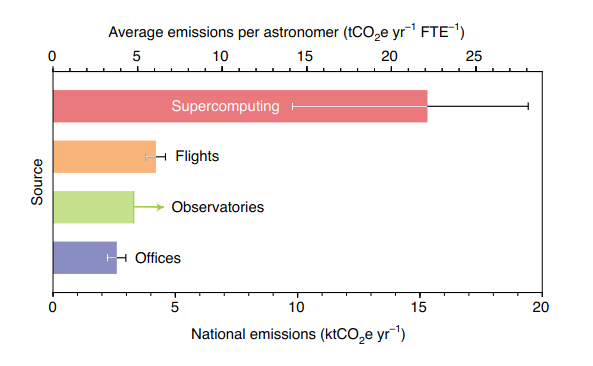
\includegraphics[width=0.75\linewidth]{supercomputing_stats.png}
    \caption{An overview of the carbon footprint of astrophysics researchers (Aujoux, Kotera and Blanchard, 2021).}
    \label{fig:enter-label}
\end{figure}

\section{Problem Statement}

PINNs have been been the subject of extensive research, with implementations in modelling nonlinear differential equations revolving around increasing accuracy (Bai 2022), reducing training times (Abbasi, 2022) and improving convergence (Bischof, 2023). The issue around the computational efficiency in approximating these differential equations hasn't been researched to the same extent. An evaluation of PINN-based methods comparative to traditional methods in terms of training times will be undertaken; in line with computational modelling of the environment. This is primarily because it's an important area that would greatly benefit from more efficient computation in modelling, and it's a field that incurs large modelling costs in general. I have chosen PINN training time as a metric for computational efficiency for this research project as it is easy to demonstrate the significant difference in the time taken to train a PINN-based model, and the time taken to approximate a solution using a traditional numerical method. When used against analysis of inference time of the PINN compared to the numerical solution, we can see the efficiency in regard to resource usage to achieve similar results accuracy wise. When it comes to environmental impact, improving the training time of PINNs could prove beneficial in regard to optimising both existing and future computational resources. 

\section{Aims and Objectives}

The primary aims of the project are:

\begin{itemize}
    \item Implement existing PINN for solving 1D linearly damped harmonic oscillator
    \item Implement secondary existing PINN to include nonlinear damping coefficient, using Van der Pol oscillator
    \item Provide performance comparison in regard to traditional methods of solving differential equations by using existing solver for numerical solution in Python.
\end{itemize}

I will begin working with two existing PINN, using code from GitHub repository at https://github.com/ben-moseley/harmonic-oscillator-pinn that approximates a solution for a 1D damped harmonic oscillator, and https://github.com/hubertbaty/PINNS-EDO2 that approximates a solution to the Van der Pol oscillator. The data of which is generated from a subset of the exact solution over the full domain in both models. This includes both the results where an ANN is trained solely using a loss function of MSE, and also where the PDE residual has been used to add prior knowledge. An extension of the original code/project forms the basis of the research project, via general implementation of the existing models and scripts relating to the implementation of numerical solutions via the SciPy library. Extending the model, to allow for the introduction on nonlinear behaviour, is a core aspect of the project. This is because of the inherent nonlinear aspect of countless physical processes that make up our climate, in which this research project revolves around in terms of modelling.

\section{Report Structure}

After specifying the problem statement, the aim and objectives, the report will then lay out the predominant research question that has arisen throughout this project. Chapter 2 will then consist of a literature review of the PINNs field; going briefly into the underlying mathematics and machine learning architecture, and then PINNs themselves and their applications. Chapter 3 revolves around the testing methodologies of the project, regarding the existing models from Ben Moseley and Hubert Baty. In Chapter 4 I will evaluate the results from these tests and provide some general analysis, with the final chapter reaching a conclusion and going over further work in the PINNs field.

\section{Research Question}

\begin{itemize}
    \item To what extent could PINNs be used to optimise large scale modelling of complex processes? 
\end{itemize}

\newpage

% ------------------------------------------------------------ %

\chapter{Literature Review}

The literature review is formed of research undertaken within the field in regard to the application of PINNs, and how these applications relate to the research questions posed in regard to improving computational efficiency. Also including background in the relevant areas of mathematics required for the understanding of these applications, and the machine learning knowledge necessary for the implementation of the physics-informed loss function and general learning process of ANNs/fully connected neural networks (FCNNs).

\section{Differential Equations}

Differential Equations, and their subsets Ordinary Differential Equations (ODEs) and Partial Differential Equations (PDEs), deal with change in regard to independent variables. The former containing ordinary derivatives, and the latter containing partial derivatives. For instance, this differential equation below is an ODE, with one independent variable 't', or time (Fangohr, 2012).

\[\frac{d^2x}{dt^2}=-\frac{k}{m}x\]

In this PDE below however, we have multiple independent variables: t, x and y (Fangohr, 2012). PDEs are specifically useful as they relate to nearly all fundamental laws of nature (Knill, 2019), revolving around combining multiple rates of change.

\[\frac{\partial u}{\partial t}=D(\frac{\partial ^2u}{\partial x^2} +\frac{\partial ^2u}{\partial y^2})\]

The relationship between differentiability and ANNs is an important one by design; as it is a desirable quality of the activation functions used in ANNs to be continuously differentiable. However, it is not completely necessary; ReLu is not differentiable at 0 and it is a very popular activation function! We will cover these methodologies in detail in 2.5.1.

\subsection{Oscillating Systems}

The subject of this research project specifically deals with approximating the solutions to two oscillating systems: a harmonic oscillator with linear damping, and the Van der Pol oscillator. These oscillating systems are of particular importance when it comes to modelling complex physical processes, and both are used in a wide variety of scientific circles: the simple harmonic oscillator can for instance be utilised in temperature models (Giorgini et al., 2021), and the Van der Pol oscillator provides a useful tool for modelling dynamical systems like glacial dynamics (Ditlevsen {\&} Ashwin, 2018).

\subsubsection{Simple Harmonic Oscillator}

\begin{quote}
    \textit{The career of a young theoretical physicist consists of treating the harmonic oscillator in ever-increasing levels of abstraction - Sidney Coleman}
\end{quote}

It is remarkable to what extent the physical processes around us are affected by harmonic motion; from a mass on a spring to the fundamental processes within quantum fields, from "atoms to oceans" (Garratt, 2020). \\

The differential equation we will be using in the baseline experiments is a second order ODE, in the form:

\[m\frac{d^2u}{dx^2}+\mu\frac{du}{dx}+ku=0\]

where \(m =\) mass, \(\mu =\) friction coefficient and \(k = \) spring constant (Moseley, 2021). \\

The introduction of damping to a simple harmonic oscillator also functions as a connective element to the system in resides in, as the reduction in oscillations via the damping coefficient will energy dissipating into the environment around it (Garratt. 2020). The conceptual simplicity of the damped harmonic oscillator, but pervasiveness of it's effect on the physical environment, makes it an excellent candidate for this research project. \\

In this specific harmonic oscillator we will be solving as a baseline, this is in an \textit{under-damped} state, which means that the spring is allowed to oscillate back and forth and the damping is slow. This is opposed to the system being overly damped or critically damped.

\subsubsection{Van der Pol Oscillator}

The Van der Pol oscillator, first introduced by Balthasar van der Pol in 1927 to describe oscillations in electrical circuits (Tsatsos, 2008), is an oscillating system with non-linear damping. The underlying mathematical equation is a second-order ODE in the form (Tsatsos, 2008):

\[\frac{d^2u}{dt^2}+\omega^2_0u-\epsilon\omega_0(1-u^2)\frac{du}{dt}=0\] \\

For this research project, the Van der Pol oscillator was a natural choice; in it's unforced form (i.e. no damping function) the equation is a form of the simple harmonic oscillator, defined as (Grimshaw, 1993):

\[\frac{d^2x}{dt^2}+x=0\]

\section{Traditional Numerical Methods}

Numerical methods for approximating solutions to PDEs are considered a 'mature' field of mathematics and engineering. Whilst we will be concentrating on a particular numerical solution (FE) to reference in terms of computational efficiency in this study; there are a core set of "well established" techniques (Suli, 2023):

\begin{itemize}
    \item finite difference methods
    \item finite element methods
    \item finite volume methods
    \item spectral methods
\end{itemize}

\section{Finite Element Method}

FEM is a numerical method for approximating solutions to various PDEs, via the subdivision of a complex/finite space into a countable and finite number of elements (Jousef Murad, 2022; Nikishkov, 2004). This is performed by a series of steps:

\begin{enumerate}
    \item Subdivision of the continuum into finite elements, into a finite element mesh
    \item Selection of the interpolation functions
    \item Finding the element properties, and establishing the matrix equation for the finite element
    \item Assembly of the element equations
\end{enumerate}

\section{Numerical Solvers in SciPy}

For the numerical solution in this research project we will be using built in functionality via the SciPy package, specifically the solve{\_}ivp functionality. This function is a useful tool for solving ODEs, so we will be using this function for both the numerical solution to the linearly damped harmonic oscillator and the Van der Pol oscillator.

\section{Machine Learning}

ML, often synonymous with artificial intelligence (AI), is made up of various statistical methods which aim to simulate human or human-like intelligence and reasoning. ML can be broadly described as a set of methods and algorithms used to extrapolate meaning from data; of which there are two primary subsets of algorithms for 'learning': unsupervised and supervised.

\subsubsection*{Supervised Algorithms}

Supervised ML algorithms work via taking data in the form of input and output variables (labelled data), and using the algorithms to "learn" or approximate the mapping function well enough for the mapping to hold given new and unseen (and unlabelled) data (Brownlee, 2023). Supervised algorithms can be further split into two classes of algorithms: classification and regression. Classification algorithms like linear classifiers or K-nearest neighbour are used to classify data into categories, and regression (e.g. linear or logistical) are used to evaluate the relationship between dependent and independent variables (IBM, 2023).

\subsubsection*{Unsupervised Algorithms}

In contrast, unsupervised algorithms rely solely on input data, and are provided with no output variables. The algorithm must rely on this input data to map out the underlying structure or distribution of the data as a whole (Brownlee, 2023). Like supervised algorithms, they can be further split into subcategories of unsupervised learning: clustering, association and dimensionality reduction. Clustering (e.g. K-means clustering) revolves around clustering data into a 'K' number of groups, association algorithms are concerned with finding relationships between data and dimensionality reduction algorithms like Principle Component Analysis are based around reducing the size of data sets via feature extraction (IBM, 2023).

\subsection{Neural Networks}

Neural networks are made up of interconnected layers of nodes, with each of these connections between the nodes maintaining a weight, which is initially randomly assigned but updated throughout the learning process. This weight dictates the strength of the connection between the two nodes, or neurons. \\ 

The backpropagation algorithm, although conceptually conceived by White and Rosenblatt with "back-coupled networks" (White and Rosenblatt, 1963), was popularised by a later paper. The concept of backpropagation was initially described as "learning rules that iteratively adjust the relative strengths of the connections", of which the goal was to adjust the weights so that the actual and desired output vectors were the same (Rumelhart, Hinton and Williams, 1986). The integration of physics-based loss into a neural network architecture makes use of the automatic differentiation that the backpropagation algorithm provides (Meng et al., 2019).

\begin{figure} [h!]
    \centering
    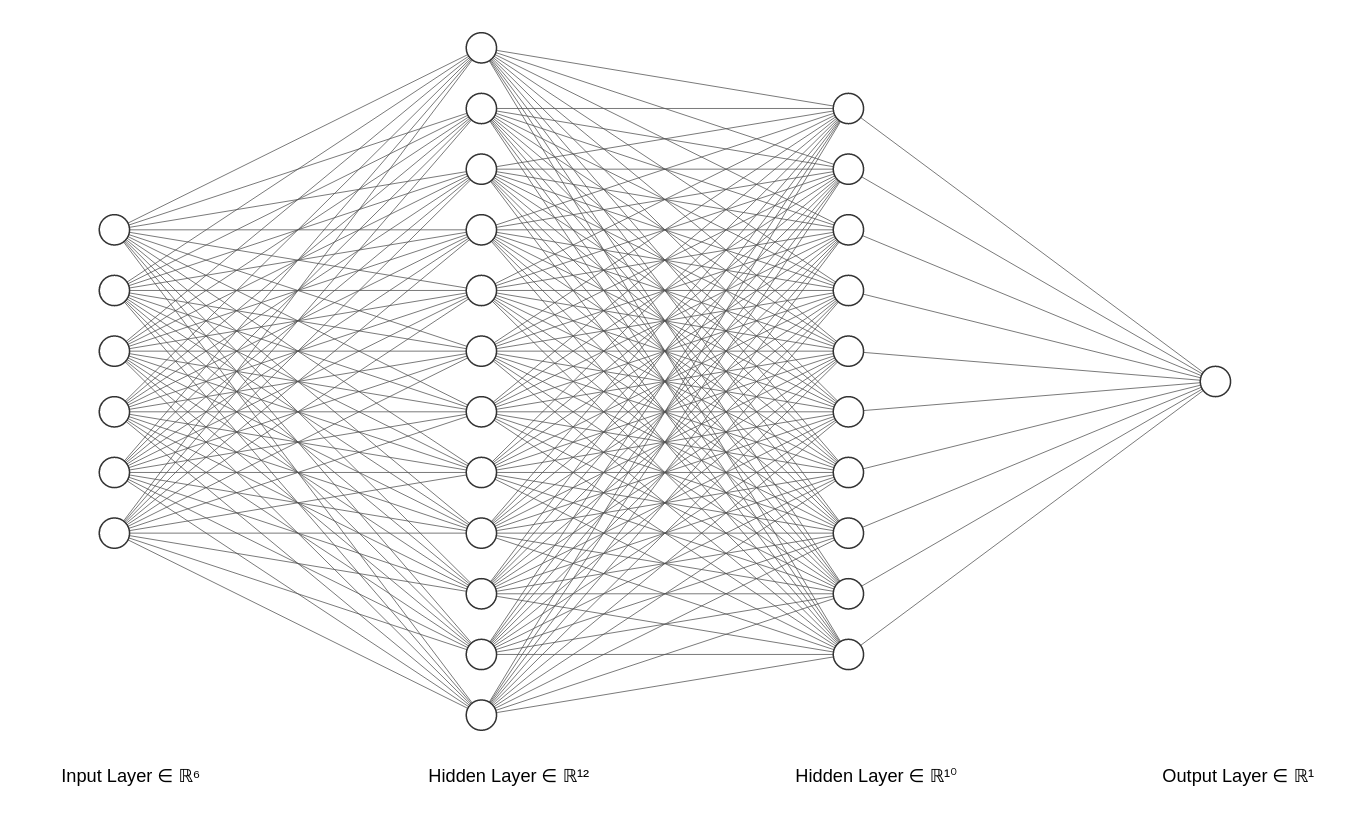
\includegraphics[width=1\linewidth]{ex1_nn.png}
    \caption{%
    FCNN with an input layer, 2 hidden layers consisting of 12 neurons and 10 neurons respectively, and an output layer. A single or dual node output layer is consistent with binary classification problems, and depends on the choice of activation function (Brownlee, 2021).}
    \label{fig:enter-label}
\end{figure}

\subsection{Physics-Informed Neural Networks}

ANNs utilise loss functions to provide a metric for evaluating the performance of the model in regards to the given data (Eusebi, 2021), with a common loss function being mean squared error (MSE). The 'job' of the neural network in regards to this loss function is \textit{minimisation} (Ambrosio, Cuomo and De Rosa, 2023). PINNs extend this implementation, and utilise the prior knowledge of physical systems by adding an extra term to the given loss function of the network, which forces the network to obey the underlying PDE outside of the given data. This is calculated via the following methodology (Moseley, 2021):

\begin{itemize}
    \item Take a set of training points from the analytical solution, and pass them through the network
    \item Calculate the gradients via automatic differentiation (autograd in PyTorch)
    \item Gradients used to calculate PDE residual
    \item Residual of PDE added to loss function as extra term
\end{itemize}

MSE as a regression-based loss function is defined as: \\

\[\min\frac{1}{N}\sum_{i}^{N} (u_{NN}(x_{i};\theta) - u_{true}(x_{i}))^2\]

In section 2.2, we defined the second order differential equation involved in the baseline code, approximating the solution to the 1D damped harmonic oscillator. We can now implement this differential equation as an added term to the loss function specified above:

\[
\min\frac{1}{N}\sum_{i}^{N} (u_{NN}(x_{i};\theta) - u_{true}(x_{i}))^2 + \frac{1}{M}\sum_{j}^{M}\left(\left[m\frac{d^2u}{dx^2}+\mu\frac{du}{dx}+ku=0\right] u_{NN}(x_{i};\theta)\right)^2
\]

where the physics loss is constructed via the underlying differential equation within the square brackets (Moseley, 2021). 

One of the major issues surrounding differential equations, specifically PDEs, is that there is a vast number where the analytical solution is intractable. However, in this case of our baseline ODE, it is known and can be given by (Moseley, 2022):

\[
u(t)=e^{-\delta t}(2A\cos(\phi + \omega t)), \hspace{10pt} \omega = \sqrt{w_{0}^2-\delta^2}
\]

There are several advantages to PINNs over traditional methods, including the ability to approximate statistical quantities for PDEs (e.g. uncertainty quantification) (Zhang et al., 2019; Yang and Perdikaris, 2019), real-time approximation (Borrel-Jensen, Engsig-Karup and Jeong, 2021; Aymerich et al, 2023), can be run directly on graphics processing units (GPUs) and are easy to parallelise via PyTorch/TensorFlow (Nvidia, 2023). This is alongside the various disadvantages of using traditional numerical methods for the approximations, like the lack of generalisation and the solving must be tailored to the specifics of a particular PDE. These qualities make PINNs a feasible candidate for approximating PDEs when it comes to reducing computational and by extension the environmental cost. \\

There is already existing research in regards to the computational efficiency of PINNs, but this is usually a side note in other areas of PINN-based research. However, this must be taken into account and has the possibility to act as a control for future experiments. In Buoso et al., 2021, the reduction in computational load was 30 fold; while this is obviously useful in small simulations or modelling, scaled to the yearly computation of a weather forecasting organisation, this is a massive reduction in carbon footprint. \\

However, PINNs are not without their disadvantages, with one of the primary disadvantages of PINNs being slower to train, less accurate, and come with convergence problems; with novel training proposals proposed to alleviate these issues (Haitsiukevich and Ilin, 2023; Krishnapriyan et al., 2021; Wang, Yu and Perdikaris, 2020; Kim et al., 2021). \\

There has also been in-depth reviews on the various extensions and types of hybrid-PINN format (Lawal et al., 2022), so this literature review will provide pointers to literature of that type instead of attempting to extend these reviews.

\section{Applications of PINNs}

PINNs were first theorised by Raissi, Perdikaris and Karniadakis (2018), in a paper that was concerned with solving time-dependent nonlinear PDEs. While using neural networks for approximating differential equations was not a new area of research (Lagaris, Likas and Fotiadis, 1998), the concept of encoding the prior knowledge of physical laws into a neural network was a novel solution. Since then, the subset of machine learning has been the subject of many different branches of research. While the models have primarily found use cases within the physical sciences, there is also promising research in areas like the medical field; finding use cases for cardiac activation mapping (Sahli Costabal et al., 2020) and building personalised biophysical models of the heart (Buoso, Joyce and Kozerke, 2021).

\begin{itemize}
    \item Within the physical sciences themselves, specifically physics, the PDEs that underpin: cosmological phase transitions PINNs (Piscopo, 2019), the time-dependent Schrodinger equation (Shah et al., 2022) and astrophysical shocks (Moschou et al., 2023) have all been solved via PINNs, with existing research in the area of Bayesian PINNs for nonlinear dynamical systems (Linka et al., 2022).
    \item In applied mathematics and engineering, PINNs have found use cases within solving heat transfer PDEs (Cai et al., 2021), solving Kolmogorov PDEs (De Ryck and Mishra, 2022), and high-speed flows (Mao, Jagtap and Karniadakis (2020).
    \item In acoustics, research has been undertaken in wave dynamics (Rasht-Behesht et al., 2021) and resonance analysis (Yokota, Kurahashi and Abe, 2023).
    \item In materials science, PINNs have been utilised for inverse problems in nanophotonics and metamaterials (Chen et al., 2020).
\end{itemize}

There has also been extensive research in uncertainty quantification (UQ), in both a classical (Zhang et al., 2019) and adversarial sense (Yang and Perdikaris, 2019). Mishra and Molinaro (2022) have also conducted research in the generalized error of PINNs. \\

In terms of extending PINNs, whilst there has been different types of PINN-based models theorised, different methodologies have been researched in terms of improving efficiency. Abbasi and Andersen (2022) have been researching physical activation functions (PAFs) as a more efficient induction of prior knowledge into the PINNs.

\section{Climate Modelling}

This brings us to a core aspect of the research project, the applications of PINNs in regard to climate modelling. As our global weather systems change and we gradually move out of the stable epoch modern society has become accustomed to, our modelling needs will potentially become more intensive:

\begin{itemize}
    \item Environmentally driven mass migration, caused by events like as sea-level rise, extreme weather events, and resource scarcity. Traditional models often struggle to capture the dynamics involved; PINNs, with their ability to incorporate physical equations into their modelling, can provide more accurate predictions of migration patterns, aiding policymakers in political driven processes like resource allocation.
    \item Enhancing early warning systems is crucial in mitigating the impact of natural disasters. These natural disasters are likely to become more common with our changing climate dynamics, and PINNs can improve the predictive capabilities of these systems by collating/combining diverse data sources, from satellite imagery to atmospheric simulations, and making sure they collectively obey the underlying physical processes involved.
    \item Climate variability has the potential to seriously impact crop yields and food security, so improving our weather modeling in the future is important. PINNs offer a means to enhance the accuracy of crop growth models by integrating the underlying physical equations regarding things like soil dynamics, plant physiology, and atmospheric interactions. This could enable both farmers and policymakers to make informed decisions around supply chains, crop selection and resource management.
\end{itemize}

\section{Python/PyTorch}

Python is a high-level, open-source interpreted programming language, created by Guido Van Rossum in the Netherlands and published in 1991. It is widely used by both amateur and professional developers across a wide variety of scientific and industrial fields; listed as a favourite language by nearly half of all developers, with Python-compatible libraries like NumPy and Pandas also featuring as favourite frameworks (Stack Overflow Developer Survey, 2023). One of the reasons Python gained popularity in the scientific community because of these libraries, as the introduction of NumPy allowed Python to compete with other languages used for data analysis purposes like R or Matlab (Thelin, 2023). \\

PyTorch is a ML library, designed for DL purposes for the fast-prototyping of models, streamlining the process from a research environment to production (Nvidia, 2023). It was originally designed by Adam Paszke as an internship project, and is built on top of the Torch library (Yasar and Lewis, 2022). Key features of PyTorch include functionality like distributed training; allowing for increased performance optimisation, and cloud support (Meta, 2023).

% ------------------------------------------------------------ %

\chapter{Implementation}

To illustrate the differences in computational efficiency between solving differential equations via physics-informed and numerical solutions, we will be using two PINN-based models and demonstrating performance using training time as a metric for computational efficiency. The ODEs we are concerned with solving are:

\begin{itemize}
    \item 1D, Second-Order Linear ODE - Damped Harmonic Oscillator
    \item 1D, Second-Order Nonlinear ODE - Van der Pol Oscillator
\end{itemize}

To evaluate the training time accurately, we will be using results gained from PINNs with no effort made to optimise the networks in regard to said training time and use a range of initial conditions:

\begin{enumerate}
    \item \textbf{Initial Position(x): x = 1.0, Initial Velocity($\frac{dx}{dt}$): $\frac{dx}{dt} = 0.0$} \\
    Default initial conditions for physics-informed model.
    \item \textbf{Initial Position(x): x = 0.0, Initial Velocity($\frac{dx}{dt}$): $\frac{dx}{dt} = -0.5$}
    Here, the oscillator starts exactly at the equilibrium position (zero displacement) with a negative initial velocity. This represents a scenario where the oscillator starts from rest at the equilibrium point but with an initial impulse in the negative direction.
    \item \textbf{Initial Position(x): x = 1.5, Initial Velocity($\frac{dx}{dt}$): $\frac{dx}{dt} = -1.5$} \\
    This choice begins the oscillator at a position significantly away from equilibrium (positive displacement) with a large negative initial velocity. It represents an initial condition where the oscillator is strongly displaced from equilibrium and has a large initial velocity directed towards the equilibrium point.
    \item \textbf{Initial Position(x): x = -0.5, Initial Velocity($\frac{dx}{dt}$): $\frac{dx}{dt} = 1.0$} \\
    This choice starts the oscillator at a negative position with a moderate initial positive velocity. It represents an initial condition where the oscillator is displaced from equilibrium in the negative direction and has a moderate initial velocity pushing it away from the equilibrium point.
\end{enumerate}
    
\section{PINN-based vs Numerical}

The PINN-based approximations to both of these differential equations are implemented via existing models; utilising FCNNs and extending them to incorporate the underlying mathematical equation. They are trained via collocation points on an analytical solution/numerical solution as training data, of which the PINN will be able to generalise outside of. The numerical solution is implemented via built-in functionality in the SciPy package, using solve{\_ivp} to provide a solution to both of the ordinary differential equations given.

% ------------------------------------------------------------ %

\chapter{Results and Analysis}

\section{Damped Harmonic Oscillator}

We first take the physics-informed model implemented via Mosely (2023) and show the training progress at regular intervals. We plot the exact solution, neural network predictions, and training data to visualize the training progress. Additionally, we plot the locations where the physics loss is calculated, helping to ensure the neural network learns the underlying physics of the system.\\

\begin{figure}[!h]
    \centering
    \begin{subfigure}[b]{0.45\linewidth}
        \centering
        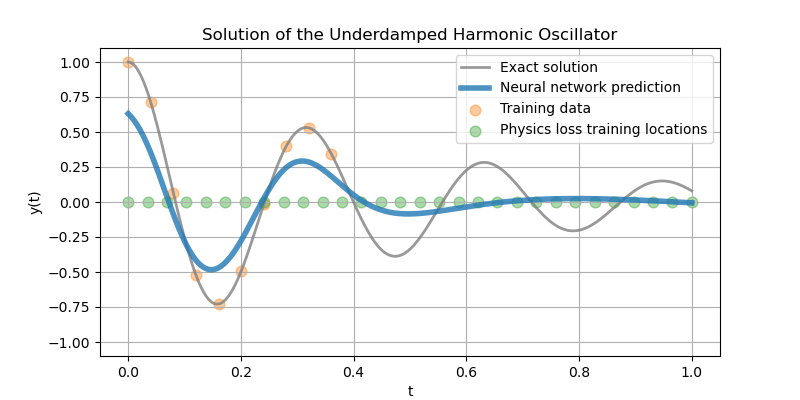
\includegraphics[width=\linewidth]{sho_4k.png}
        \caption{4k iterations}
        \label{subfig:figure1}
    \end{subfigure}
    \hfill
    \begin{subfigure}[b]{0.45\linewidth}
        \centering
        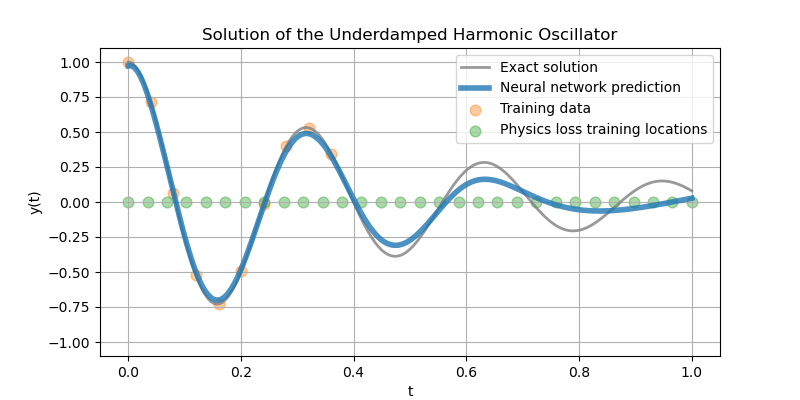
\includegraphics[width=\linewidth]{sho_8k.png}
        \caption{8k iterations}
        \label{subfig:figure2}
    \end{subfigure}
    \vskip\baselineskip
    \begin{subfigure}[b]{0.45\linewidth}
        \centering
        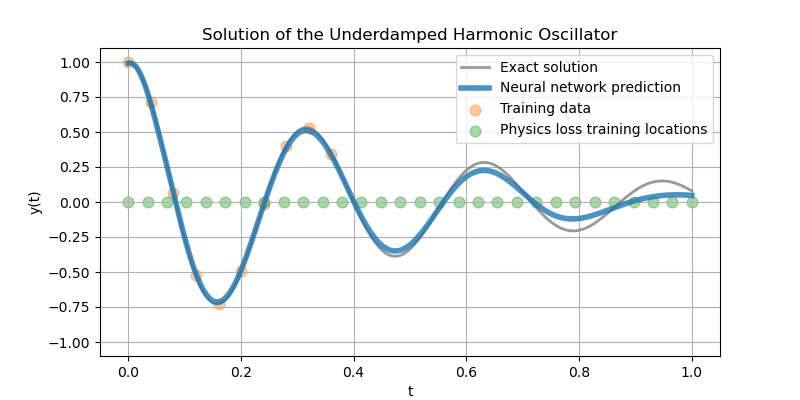
\includegraphics[width=\linewidth]{sho_12k.png}
        \caption{12k iterations}
        \label{subfig:figure3}
    \end{subfigure}
    \hfill
    \begin{subfigure}[b]{0.45\linewidth}
        \centering
        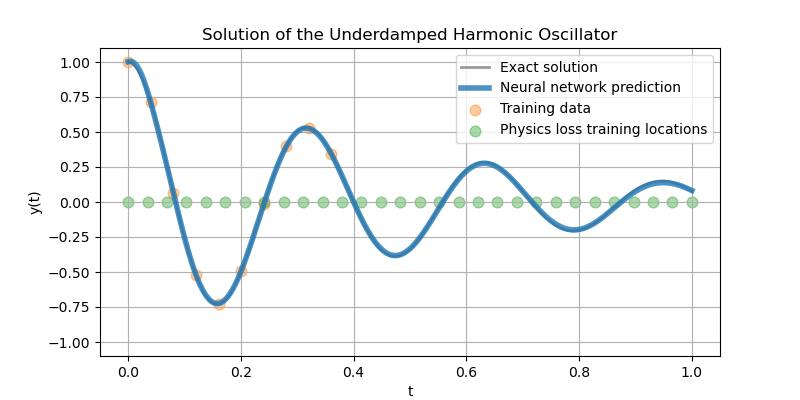
\includegraphics[width=\linewidth]{sho_16k.png}
        \caption{16k iterations}
        \label{subfig:figure4}
    \end{subfigure}
    \caption{Physics-informed solution for the linearly damped 1D harmonic oscillator.}
    \label{fig:overall_label}
\end{figure}

\section{Van Der Pol Oscillator}

In the PINN concerned with approximating the solution to the solution to the Van der Pol oscillator, we first visualise the exact solution and the phase space of the oscillator. \\

\begin{figure}[!h]
    \centering
    \begin{subfigure}[b]{0.45\linewidth}
        \centering
        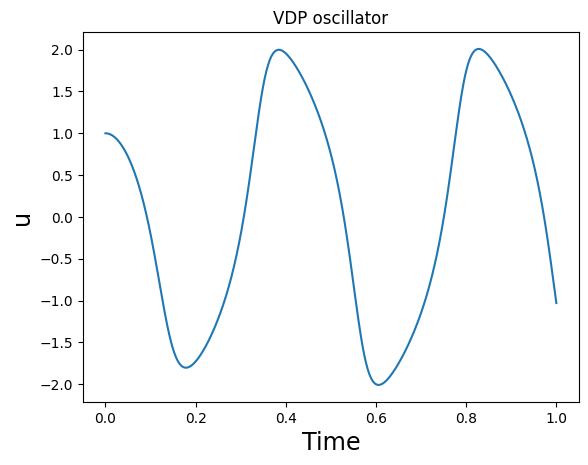
\includegraphics[width=\linewidth]{vdp.png}
        \label{subfig:figure1}
    \end{subfigure}
    \hfill
    \begin{subfigure}[b]{0.45\linewidth}
        \centering
        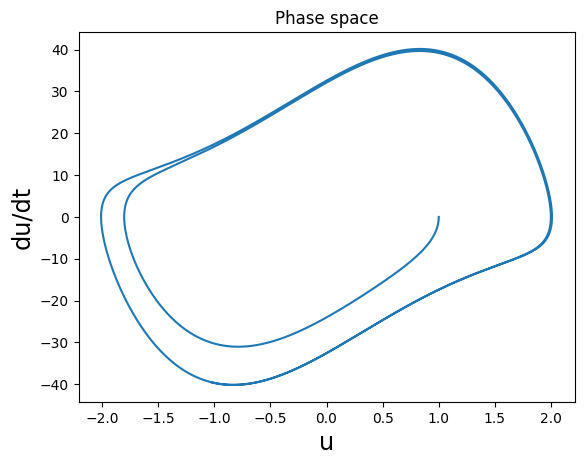
\includegraphics[width=\linewidth]{vdp_phasespace.png}
        \label{subfig:figure2}
    \end{subfigure}
    \caption{Exact solution and phase space for Van Der Pol oscillator.}
    \label{fig:overall_label}
\end{figure}

In this model however, we can demonstrate the limitations of using a standard neural network when it comes to approximating these solutions. In figure 4.3, we can see how the model performs well on the part of the solution where training points are given, but is unable to generalise outside of the given training data. This is a core part of what makes physics-informed models a viable solution for approximating differential equations rather than standard neural networks; with limited data, the PINN-based models are able to generalise in the absence of complete data. \\

\begin{figure}[!h]
    \centering
    \begin{subfigure}[b]{0.45\linewidth}
        \centering
        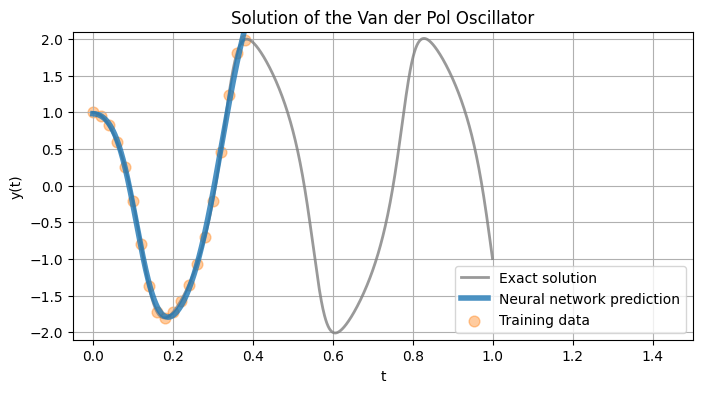
\includegraphics[width=\linewidth]{vdp_nn4k.png}
        \caption{4k iterations}
        \label{subfig:figure1}
    \end{subfigure}
    \hfill
    \begin{subfigure}[b]{0.45\linewidth}
        \centering
        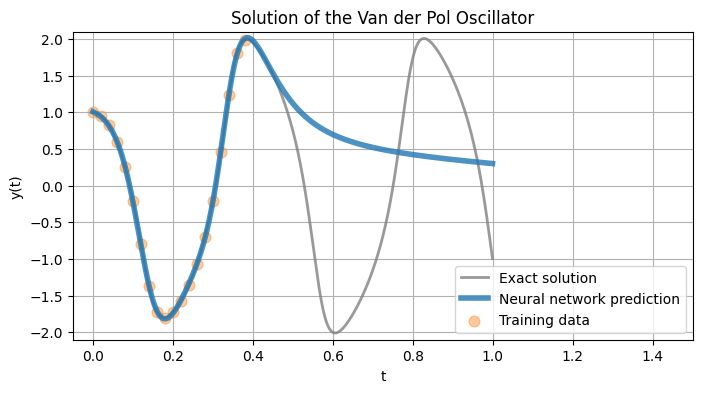
\includegraphics[width=\linewidth]{vdp_nn8k.png}
        \caption{8k iterations}
        \label{subfig:figure2}
    \end{subfigure}
    \vskip\baselineskip
    \begin{subfigure}[b]{0.45\linewidth}
        \centering
        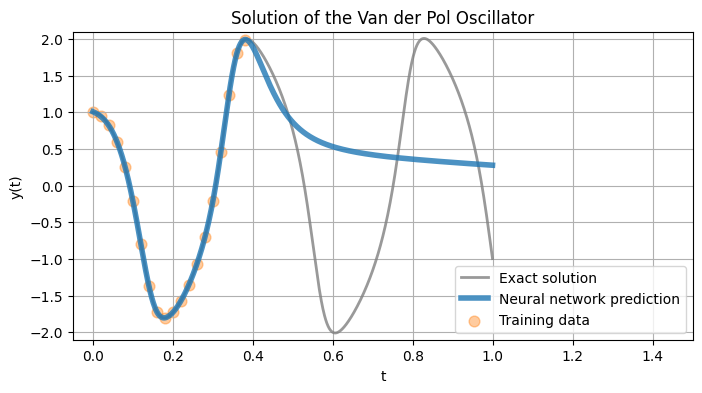
\includegraphics[width=\linewidth]{vdp_nn12k.png}
        \caption{12k iterations}
        \label{subfig:figure3}
    \end{subfigure}
    \hfill
    \begin{subfigure}[b]{0.45\linewidth}
        \centering
        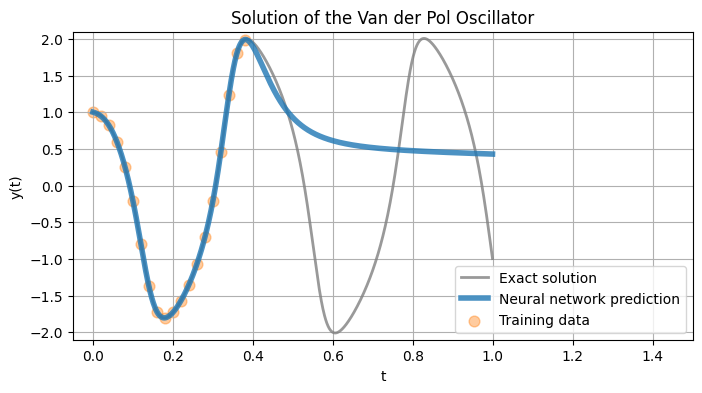
\includegraphics[width=\linewidth]{vdp_nn16k.png}
        \caption{16k iterations}
        \label{subfig:figure4}
    \end{subfigure}
    \caption{Standard neural network solution for the Van Der Pol oscillator.}
    \label{fig:overall_label}
\end{figure}

In the physics-informed approximation however, in figure 4.4, we're able to see how even with the same training points, the extended neural network is performs far better outside the training data. \\ 

\begin{figure}[!h]
    \centering
    \begin{subfigure}[b]{0.45\linewidth}
        \centering
        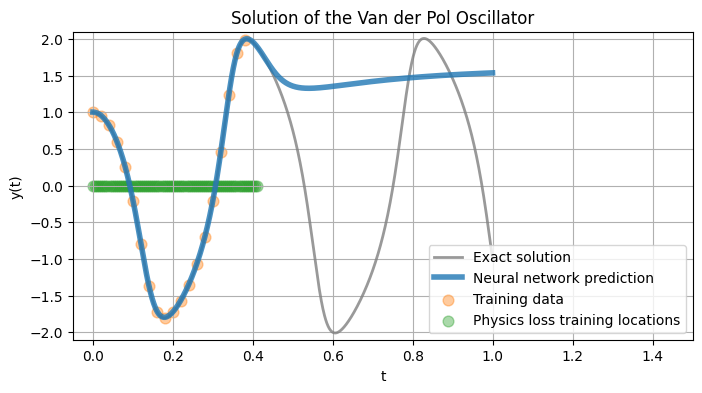
\includegraphics[width=\linewidth]{vdp_12k.png}
        \caption{12k iterations}
        \label{subfig:figure1}
    \end{subfigure}
    \hfill
    \begin{subfigure}[b]{0.45\linewidth}
        \centering
        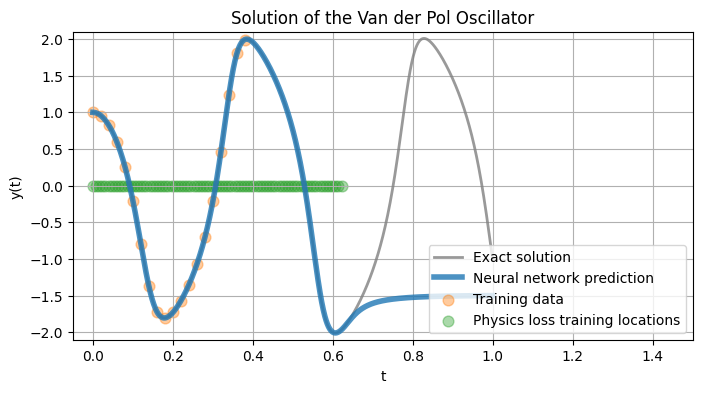
\includegraphics[width=\linewidth]{vdp_24k.png}
        \caption{24k iterations}
        \label{subfig:figure2}
    \end{subfigure}
    \vskip\baselineskip
    \begin{subfigure}[b]{0.45\linewidth}
        \centering
        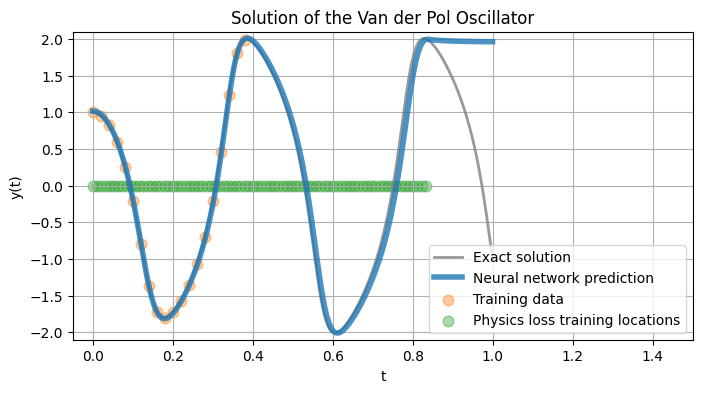
\includegraphics[width=\linewidth]{vdp_32k.png}
        \caption{36k iterations}
        \label{subfig:figure3}
    \end{subfigure}
    \hfill
    \begin{subfigure}[b]{0.45\linewidth}
        \centering
        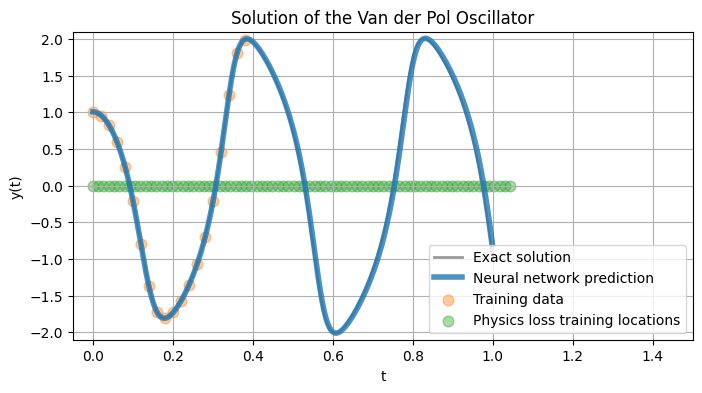
\includegraphics[width=\linewidth]{vdp_44k.png}
        \caption{48k iterations}
        \label{subfig:figure4}
    \end{subfigure}
    \caption{Physics-informed solution solution for the Van der Pol oscillator.}
    \label{fig:overall_label}
\end{figure}

\section{Results}

As we can see from the results below, the training time involved with a physics-informed solution is one of the key issues when approximating these complex mathematical equations. The vast time difference between training time of PINNs and the time taken for  a numerical solver to gain the same result is arguably a key reason the scientific community is reluctant to move away from traditional methods. However, the inference time of the PINN, and the time taken to approximate a numerical solution via solve{\_ivp}, in this particular testing case has a worst case time difference of 0.005 and 0.001 in the best case. Improving training times of PINNs is an active area of research, but it is important to reiterate the statement from Raissi, Perdikaris and Karniadakis (2018) that one of the more promising use cases when it comes to PINNs is not to replace the faster (and more accurate) numerical solutions, but to augment them. However, the potentially negligible time differences in inference time and the time taken for a numerical solver to approximate a solution does prove promising.

\begin{table}[h!]
\centering
\begin{tabular}{||c c c c c|} 
 \hline
  System & Initial Conditions & Training & Inference & Numerical \\ [0.5ex] 
 \hline\hline
 Harmonic Oscillator & x=1.0, v=0.0 & 48.773 & 0.010 & 0.006 \\
 Van Der Pol Oscillator & x=1.0, v=0.0 & 455.211 & 0.015 & 0.012 \\ 
 Van Der Pol Oscillator & x=0.0, v=-0.5 & 409.927 & 0.014 & 0.013 \\ 
 Van Der Pol Oscillator & x=1.5, v=-1.5 & 408.185 & 0.010 & 0.015 \\ 
 Van Der Pol Oscillator & x=-0.5, v=1.0 & 414.772 & 0.012 & 0.010 \\ [1ex] 
 \hline
\end{tabular}
\caption{Comparison of training/inference times of the two systems, comparative to equivalent python code using a numerical solver.}
\label{table:1}
\end{table}

\section{Conclusion}

Physics-Informed Neural Networks have the potential to provide a viable solution to some of the most difficult modelling problems we face as a society. If we were able to reduce the computational load via a reduction in training time when it came to physics-informed solutions, they could prove very useful in instances where there is limited data but an accurate solution is necessary. As mentioned previously, the data gathered by Buoso et al., 2021, showed a 30 fold reduction in computational load via reduction in compute time compared to finite element; the benefits of PINNs are non-negligible at small scale, and have the potential to save a significant amount of money, power and water usage when it comes to modelling the complex processes involved in climate processes. \\

Future research could involve a further study into how physics-informed solutions could augment existing numerical solutions; much of the research involved in PINNs revolves around improving PINN training or convergence issues with the physics-informed models. Research could also revolve around potential areas where physics-informed solutions could be of the most benefit; small subsets of existing problems where a numerical solver is unnecessary. Resource optimisation is going to become more of an issue as: our demand increases, we create more powerful machine learning models and our climate becomes ever more chaotic. The introduction of PINNs into standardised modelling processes could provide the solution to resource optimisation problems that we might face in the future.

% ------------------------------------------------------------ %

\chapter{References}

Abbasi, J. and Andersen, P.Ø. (2022) Physical Activation Functions (pafs): An approach for more efficient induction of physics into physics-informed Neural Networks (pinns), arXiv.org. Available at: https://arxiv.org/abs/2205.14630v1 (Accessed: 11 November 2023). \\

Alshanti, W.G. et al. (2023) ‘A novel analytical approach for solving partial differential equations via a tensor product theory of Banach spaces’, Partial Differential Equations in Applied Mathematics, 8, p. 100531. doi:10.1016/j.padiff.2023.100531. \\

Ambrosio, P., Cuomo, S. and De Rosa, M. (2023) A physics-informed deep learning approach for solving strongly degenerate parabolic problems, arXiv.org. Available at: https://arxiv.org/abs/2310.00172 (Accessed: 11 November 2023). \\

Aujoux, C., Kotera, K. and Blanchard, O. (2021) ‘Estimating the carbon footprint of the Grand Project, a multi-decade astrophysics experiment’, Astroparticle Physics, 131, p. 102587. doi:10.1016/j.astropartphys.2021.102587. \\

Aymerich, E. et al. (2023) ‘Physics informed neural networks towards the real-time calculation of heat fluxes at W7-X’, Nuclear Materials and Energy, 34, p. 101401. doi:10.1016/j.nme.2023.101401. \\

Bai, G. (2021) ‘Physics informed Neural Networks (pinns) for approximating nonlinear dispersive pdes’, Journal of Computational Mathematics, 39(6), pp. 816–847. doi:10.4208/jcm.2101-m2020-0342. \\

Baty, H. (2023) Solving stiff ordinary differential equations using physics informed neural networks (pinns): Simple recipes to improve training of vanilla-pinns, arXiv.org. Available at: https://arxiv.org/abs/2304.08289 (Accessed: 28 April 2024). \\

Bischof, R. (2023) Improving physics-informed neural networks through adaptive loss balancing, Medium. Available at: https://towardsdatascience.com/improving-pinns-through-adaptive-loss-balancing-55662759e701 (Accessed: 27 November 2023). \\

Borrel-Jensen, N., Engsig-Karup, A.P. and Jeong, C.-H. (2021) Physics-informed Neural Networks (pinns) for sound field predictions with parameterized sources and impedance boundaries, arXiv.org. Available at: https://arxiv.org/abs/2109.11313v2 (Accessed: 13 November 2023). \\

Brownlee, J. (2021) How to choose an activation function for deep learning, MachineLearningMastery.com. Available at: https://machinelearningmastery.com/choose-an-activation-function-for-deep-learning/ (Accessed: 12 November 2023). \\

Brunton, S.L. and Kutz, J.N. (2023) Machine learning for partial differential equations, arXiv.org. Available at: https://arxiv.org/abs/2303.17078 (Accessed: 13 November 2023). \\

Buoso, S., Joyce, T. and Kozerke, S. (2021) ‘Personalising left-ventricular biophysical models of the heart using parametric physics-informed neural networks’, Medical Image Analysis, 71, p. 102066. doi:10.1016/j.media.2021.102066. \\

Cai, S. et al. (2021) ‘Physics-informed neural networks for heat transfer problems’, Journal of Heat Transfer, 143(6). doi:10.1115/1.4050542. \\

Chen, Y. et al. (2020) ‘Physics-informed neural networks for inverse problems in Nano-optics and Metamaterials’, Optics Express, 28(8), p. 11618. doi:10.1364/oe.384875. \\

Copenhagen Centre on Energy Efficiency (2020). Greenhouse gas emissions in the ICT sector. Available at: https://c2e2.unepccc.org/wp-content/uploads/sites/3/2020/03/green \\ house-gas-emissions-in-the-ict-sector.pdf (Accessed: 22 November 2023). \\

Cuomo, S. et al. (2022) ‘Scientific machine learning through physics–informed Neural Networks: Where we are and what’s next’, Journal of Scientific Computing, 92(3). doi:10.1007/s10915-022-01939-z. \\

De Ryck, T. and Mishra, S. (2022) ‘Error analysis for physics-informed Neural Networks (pinns) approximating Kolmogorov pdes’, Advances in Computational Mathematics, 48(6). doi:10.1007/s10444-022-09985-9. \\

Ditlevsen, P.D. and Ashwin, P. (2018) ‘Complex climate response to astronomical forcing: The middle-pleistocene transition in glacial cycles and changes in frequency locking’, Frontiers in Physics, 6. doi:10.3389/fphy.2018.00062. \\

Eusebi, R. (2021) Physics-Informed Neural Networks for Tropical Cyclone 2D Flow Reconstruction. Available at: https://www.pacm.princeton.edu/sites/default/files/2{\_}page{\_}sum- \\ mary-eusebi{\_}pinn{\_}2dcase.pdf (Accessed: 26 November 2023). \\

Fangohr, H. (2012) Solving partial differential equations (pdes) - University of Southampton. Available at: https://www.southampton.ac.uk/~fangohr/teaching/comp6024/comp6- \\ 024-pdes.pdf (Accessed: 13 November 2023). \\

Garrett, S.L. (2020) ‘The simple harmonic oscillator’, Understanding Acoustics, pp. 59–131. \\ doi:10.1007/978-3-030-44787-8{\_}2. \\

Gao, H., Wang, J.-X. and Zahr, M.J. (2020) ‘Non-intrusive model reduction of large-scale, nonlinear dynamical systems using Deep Learning’, Physica D: Nonlinear Phenomena, 412, p. 132614. doi:10.1016/j.physd.2020.132614. \\

Giorgini, A., Mamon, R.S. and Rodrigo, M.R. (2021) ‘A stochastic harmonic oscillator temperature model for the valuation of weather derivatives’, Mathematics, 9(22), p. 2890. doi:10.3390/math9222890. \\

Grimshaw, R., Nonlinear ordinary differential equations, CRC Press, 153–163, (1993), ISBN 0-8493-8607-1. \\

Grossmann, T.G. et al. (2023) Can physics-informed neural networks beat the finite element method?, arXiv.org. Available at: https://arxiv.org/abs/2302.04107 (Accessed: 26 November 2023). \\

Guo, J. et al. (2023) ‘Pre-training strategy for solving evolution equations based on physics-informed Neural Networks’, Journal of Computational Physics, 489, p. 112258. doi:10.1016/j.jcp.2023.112258. \\

Haitsiukevich, K. and Ilin, A. (2023) Improved training of physics-informed neural networks with model ensembles, arXiv.org. Available at: https://arxiv.org/abs/2204.05108 (Accessed: 22 November 2023). \\

Jeppesen, J. (2022) Fact sheet: Supercomputing at ECMWF, ECMWF. Available at: https://www.ecmwf.int/en/about/media-centre/focus/2022/fact-sheet-supercomputing-ecmwf (Accessed: 27 November 2023). \\

Jousef Murad (2022) The finite element method (FEM) – A beginner’s guide, Jousef Murad. Available at: https://www.jousefmurad.com/fem/the-finite-element-method-beginners-guide/ (Accessed: 13 November 2023). \\

Karniadakis, G.E. et al. (2021) ‘Physics-informed Machine Learning’, Nature Reviews Physics, 3(6), pp. 422–440. doi:10.1038/s42254-021-00314-5. \\

Kim, S. (2023) Numerical methods for partial differential equations. Available at: \\ https://skim.math.msstate.edu/LectureNotes/NumerPDEs{\_}Lecture.pdf (Accessed: \\ 11 November 2023). \\

Kim, J. et al. (2021) ‘DPM: A novel training method for physics-informed neural networks in extrapolation’, Proceedings of the AAAI Conference on Artificial Intelligence, 35(9), pp. 8146–8154. doi:10.1609/aaai.v35i9.16992. \\

Knill, O. (2019) A Lecture on Partial Differential Equations, A lecture on partial differential equations. Available at: https://people.math.harvard.edu/~knill/pedagogy/pde/index.html (Accessed: 27 November 2023). \\

Krishnapriyan, A.S. et al. (2021) Characterizing possible failure modes in physics-informed Neural Networks, arXiv.org. Available at: https://arxiv.org/abs/2109.01050 (Accessed: 22 November 2023). \\

Lagaris, I.E., Likas, A. and Fotiadis, D.I. (1998) ‘Artificial neural networks for solving ordinary and partial differential equations’, IEEE Transactions on Neural Networks, 9(5), pp. 987–1000. doi:10.1109/72.712178. \\

Lannelongue, L. et al. (2021) ‘Ten simple rules to make your computing more environmentally sustainable’, PLOS Computational Biology, 17(9). doi:10.1371/journal.pcbi.1009324. \\

Lawal, Z.K. et al. (2022) ‘Physics-informed Neural Network (PINN) evolution and beyond: A systematic literature review and Bibliometric analysis’, Big Data and Cognitive Computing, 6(4), p. 140. doi:10.3390/bdcc6040140. \\

Linka, K. et al. (2022) Bayesian physics-informed Neural Networks for real-world nonlinear dynamical systems, arXiv.org. Available at: https://doi.org/10.48550/\\arXiv.2205.08304 (Accessed: 11 November 2023). \\

Mao, Z., Jagtap, A.D. and Karniadakis, G.E. (2020) ‘Physics-informed neural networks for high-speed flows’, Computer Methods in Applied Mechanics and Engineering, 360, p. 112789. doi:10.1016/j.cma.2019.112789. \\

Meng, X. et al. (2019) ‘PPINN: Parareal physics-informed neural network for time-dependent pdes’, Computer Methods in Applied Mechanics and Engineering, 370, p. 113250. doi:10.1016/j.cma.2020.113250. \\

Metrics and scoring: Quantifying the quality of predictions (no date) scikit. Available at: https://scikit-learn.org/stable/modules/model{\_}evaluation.html (Accessed: 12 November 2023). \\

Mishra, S. and Molinaro, R. (2022) ‘Estimates on the generalization error of physics-informed neural networks for approximating pdes’, IMA Journal of Numerical Analysis, 43(1), pp. 1–43. doi:10.1093/imanum/drab093. \\

Moschou, S.P. et al. (2023) ‘Physics-informed neural networks for modeling astrophysical shocks’, Machine Learning: Science and Technology, 4(3), p. 035032. doi:10.1088/2632-2153/acf116. \\

Moseley, B. (2022) PINN Intro Workshop, GitHub. Available at: https://github.com/ben-moseley/harmonic-oscillator-pinn-workshop/blob/main/PINN{\_}intro{\_}workshop.ipynb (Accessed: 27 November 2023). \\

Moseley, B. (2023) So, what is a physics-informed neural network?, Ben Moseley. Available at: https://benmoseley.blog/my-research/so-what-is-a-physics-informed-neural-net-work/ (Accessed: 13 November 2023). \\

Nikishkov, G.P. (2004) Introduction to the Finite Element Method. Available at: \\ https://www.iitg.ac.in/mech/documents/128/introfem.pdf (Accessed: 13 November 2023). \\

NOAA (no date) Climate forcing, NOAA Climate.gov. Available at: https://www.climat- \\ e.gov/maps-data/climate-data-primer/predicting-climate/climate-forcing (Accessed: 27 November 2023). \\

Piscopo, M.L., Spannowsky, M. and Waite, P. (2019) Solving differential equations with neural networks: Applications to the calculation of cosmological phase transitions, \\ arXiv.org. Available at: https://arxiv.org/abs/1902.05563 (Accessed: 10 November 2023). \\

Pytorch (2023) Meta Open Source. Available at: https://opensource.fb.com/projects/py- \\ torch/ (Accessed: 24 November 2023). \\

Qian, Y. et al. (2023) ‘Physics-informed neural networks for approximating dynamic (hyperbolic) pdes of second order in time: Error Analysis and algorithms’, Journal of Computational Physics, 495, p. 112527. doi:10.1016/j.jcp.2023.112527. \\

Raissi, M., Perdikaris, P. and Karniadakis, G.E. (2019) ‘Physics-informed Neural Networks: A deep learning framework for solving forward and inverse problems involving nonlinear partial differential equations’, Journal of Computational Physics, 378, pp. 686–707. doi:10.1016/j.jcp.2018.10.045. \\

Raissi, M., Perdikaris, P. and Karniadakis, G.E. (2017) Physics informed Deep Learning (part I): Data-driven solutions of nonlinear partial differential equations, arXiv.org. Available at: https://arxiv.org/abs/1711.10561 (Accessed: November 2023). \\

Raissi, M. and Karniadakis, G.E. (2018) ‘Hidden physics models: Machine learning of nonlinear partial differential equations’, Journal of Computational Physics, 357, pp. 125–141. doi:10.1016/j.jcp.2017.11.039. \\

Rasht-Behesht, M. et al. (2021) Physics-informed Neural Networks (pinns) for wave propagation and full waveform inversions [Preprint]. doi:10.1002/essoar.10507871.1. \\

Rumelhart, D.E., Hinton, G.E. and Williams, R.J. (1986) ‘Learning representations by back-propagating errors’, Nature, 323(6088), pp. 533–536. doi:10.1038/323533a0. \\

Sahli Costabal, F. et al. (2020) ‘Physics-informed neural networks for cardiac activation mapping’, Frontiers in Physics, 8. doi:10.3389/fphy.2020.00042. \\

Schwartz, M. (no date) Matthew Schwartz lecture 1: Simple harmonic oscillators. Available at: https://scholar.harvard.edu/files/schwartz/files/lecture1-oscillators-and-\\ linearity.pdf (Accessed: 27 October 2023). \\

Shah, K. et al. (2022) Physics-informed neural networks as solvers for the time-dependent Schrödinger equation, arXiv.org. Available at: https://arxiv.org/abs/2210.12522 (Accessed: 11 November 2023). \\

Stack overflow developer survey 2023 (no date) Stack Overflow. Available at: \\ https://survey.stackoverflow.co/2023/ (Accessed: 22 November 2023). \\

Stevens, A.R. et al. (2020) ‘The imperative to reduce carbon emissions in astronomy’, Nature Astronomy, 4(9), pp. 843–851. doi:10.1038/s41550-020-1169-1. \\

Stiasny, J., Chevalier, S. and Chatzivasileiadis, S. (2021) ‘Learning without data: Physics-informed neural networks for fast time-domain simulation’, 2021 IEEE International Conference on Communications, Control, and Computing Technologies for Smart Grids (SmartGridComm) [Preprint]. doi:10.1109/smartgridcomm51999.2021.9631995. \\

Strubell, E., Ganesh, A. and McCallum, A. (2019) ‘Energy and policy considerations for Deep Learning in NLP’, Proceedings of the 57th Annual Meeting of the Association for Computational Linguistics [Preprint]. doi:10.18653/v1/p19-1355. \\

Suli, E. (no date) Numerical solution of partial differential equations. Available at: https://people.maths.ox.ac.uk/suli/PCAM{\_}Numerical{\_}Solution{\_}of{\_}PDEs.pdf (Accessed: 27 November 2023). \\

Thelin, R. (2023) Python version history: How python has changed over the years, Educative. Available at: https://www.educative.io/blog/python-versions-history (Accessed: 23 November 2023). \\

Tollefson, J. (2023) ‘Climate scientists push for access to world’s biggest supercomputers to build better Earth models’, Nature [Preprint]. doi:10.1038/d41586-023-02249-6. \\

Tsatsos, M. (2008) The van der pol equation, arXiv.org. Available at: https://doi.org/10.48550/arXiv.0803.1658 (Accessed: 28 April 2024). \\

Wang, S. et al. (2023) An expert’s guide to training physics-informed Neural Networks, arXiv.org. Available at: https://arxiv.org/abs/2308.08468 (Accessed: 10 November 2023). \\

Wang, S., Yu, X. and Perdikaris, P. (2020) When and why pinns fail to train: A neural tangent kernel perspective, arXiv.org. Available at: https://arxiv.org/abs/2007.14527 (Accessed: 22 November 2023). \\

What is supervised learning? (no date) IBM. Available at: \\ https://www.ibm.com/topics/supervised-learning (Accessed: 22 November 2023). \\

What is unsupervised learning? (no date) IBM. Available at: \\ https://www.ibm.com/topics/unsupervised-learning (Accessed: 22 November 2023). \\

NVIDIA. What is pytorch? (no date) NVIDIA Data Science Glossary. Available at: \\ https://www.nvidia.com/en-us/glossary/data-science/pytorch/ (Accessed: 13 November 2023). \\

White, B.W. and Rosenblatt, F. (1963) ‘Principles of Neurodynamics: Perceptrons and the theory of Brain Mechanisms’, The American Journal of Psychology, 76(4), p. 705. doi:10.2307/1419730. \\

Yang, Y. and Perdikaris, P. (2019) ‘Adversarial uncertainty quantification in physics-informed Neural Networks’, Journal of Computational Physics, 394, pp. 136–152. \\ doi:10.1016/j.jcp.2019.05.027. \\

Yasar, K. and Lewis, S. (2022) What is pytorch?, Enterprise AI. Available at: \\ https://www.techtarget.com/searchenterpriseai/definition/PyTorch (Accessed: 24 November 2023). \\

Yokota, K., Kurahashi, T. and Abe, M. (2023) Physics-informed neural network for acoustic resonance analysis, arXiv.org. Available at: https://arxiv.org/abs/2310.11804 (Accessed: 11 November 2023). \\

Zhang, D. et al. (2019) ‘Quantifying total uncertainty in physics-informed neural networks for solving forward and inverse stochastic problems’, Journal of Computational Physics, 397, p. 108850. doi:10.1016/j.jcp.2019.07.048.  \\

% ------------------------------------------------------------ %

\chapter{Computation}

\section{Sampling}

\section{PINN Architecture}

\section{Software}

The FCNN, and subsequent PINN, were both implemented in the ML framework PyTorch. For ML logging purposes and visualisation of FCNN execution graphs, I used matplotlib, Google Colab and Torchviz respectively. For visualisation of the actual NN architecture I used a web-based tool at: https://alexlenail.me/NN-SVG/index.html.

\section{Hardware}

All experiments and testing were undertaken on a Dell XPS laptop: 7.5GB memory, Intel Core i5-8250C CPU @ 1.6GHz x 4, and Intel graphics card UHD Graphics 620. The linux kernel is 6.1.44-1-Manjaro.

\end{document}